\documentclass[10pt]{article}
\usepackage{fullpage,amsthm,amsmath,amssymb,enumitem,url,verbatim,graphicx}
\usepackage{color}
\usepackage{biblatex}
\usepackage{titlesec}
\usepackage{listings}
\usepackage{booktabs}

\addbibresource{references.bib}

\begin{document}

\title{\Large CS 267 Project: Parallelizing Cartesian Tree Construction \\ 
on Multiple Nodes with Partitioned Global Address Space}
\author{\large Andrew Head}
\date{}
\maketitle

% Section resizing hint from
% http://tex.stackexchange.com/questions/103286/how-to-change-section-subsection-font-size
\titleformat{\section}{\normalfont\fontsize{10}{11}\bfseries}{\thesection}{1em}{}

% \pagenumbering{gobble}

\vspace{-5ex}

\section{Introduction}

This project focuses on adapting an existing parallel algorithm for Cartesian tree construction to
a new parallel architecture: partitioned global address space (PGAS).
We report on a simple but elegant adaptation of the algorithm to PGAS\@.
We describe the key insight---that memory access can be kept mostly local for this
divide-and-conquer algorithm---that motivates our implementation.
Although we fail to outperform the existing technique, we report evidence of sublinear strong and
weak scaling for our adaptation, even with multiple nodes (while the original algorithm could run
on only one node).
We describe techniques that we believe may enable performance beyond the baseline algorithm.

\subsection{Motivation}

% The inspiration for this project came from an unlikely source.
The first author's past research focused on automatically generating explanations of
micro-languages like regular expressions~\cite{head_tutorons_2015}.
His aim in this work was to develop a pipeline that would take in arbitrary regular expressions and generate
realistic, readable examples strings of what it matched.

The algorithm we focus on here---Cartesian tree construction, as a first step in suffix tree
construction---was the component of this pipeline where the author found
the most feasible and interesting potential for parallelization using course concepts.
Certain parts of the pipeline, including regular expression matching, are not simple to optimize
beyond ``embarrassingly parallel'' improvements:
Asanovic et al.~\cite{asanovic_view_2009} points out that only `work-inefficient' algorithms are
known for executing finite state machines.
Algorithms have been proposed for improving the speed of regular expression matching through
novel processor architectures (e.g.,~\cite{brodie_scalable_2006}), the use of graphics processing
(e.g.,~\cite{vasiliadis_regular_2009}), splitting input for specific matching
problems~\cite{jones_parallelizing_2009}, and a parallel prefix oriented approach to matching
strings~\cite{hillis_data_1986}.
However, the first author found that, in practice, regular expression matching seemed to be
I/O-bound rather than computation-bound.

While it is not necessarily the bottleneck to the system, an interesting potential resided in
the problem of building a suffix tree at a faster speed.
Initial tests with a 10M file revealed that suffix tree construction with a state-of-the-art
algorithm~\cite{shun_simple_2014} was too slow for interactive automatic explanation speeds---
about two-tenths of a second.
So we set out to improve the speed of this component, particularly because we thought there would
be an interesting problem in refactoring the parallel architecture for the algorithm.
Suffix tree construction is also an active area of research, and it has been for some time.
Suffix trees can provide a fast, often linear-time solution to many string-related problems, 
including finding maximal repeated substrings~\cite{gusfield_algorithms_1997}, making them quite
useful for applications including processing biological sequence
data~\cite{bieganski_generalized_1994}.

\subsection{Related work}

Algorithms for constructing suffix trees have been around for a long time.
Perhaps one of the most-taught algorithms is Ukkonen's, a linear time algorithm for constructing
suffix trees~\cite{ukkonen_online_1995}.
Since Ukkonen, there have been a number of algorithms that have sought to gain even better
performance with the use of parallel tree construction.
The approaches and contexts of each algorithm varies.
I review a set of very recent approaches to provide an overview.
Tsirogiannis et al.\ describe a cache-conscious algorithm tailored to chip-multiprocessor
architectures~\cite{tsirogiannis_suffix_2010}.
Mansour et al.\ develop serial and parallel disk-based suffix tree construction algorithms
optimized to perform well when the string cannot fit completely in main memory~\cite{mansour_era_2011}.
Shun \& Blelloch~\cite{shun_simple_2014} propose the algorithm on which this work is based.
They claim that their algorithm runs in $O\left(\min{d \log n, n}\right)$ time, 
with tree height $d$.
We seek to add a divisor to this runtime, to achieve runtime of
$O\left(\min{\frac{d}{p} \log n, \frac{n}{p}}\right)$.
We are not completely successful in this effort, but we make a first step.

We use their algorithm as a starting point, asking how we can extend their multi-thread single-node
code to run more efficiently on multiple nodes with multiple threads.
In contrast to the other mentioned work~\cite{tsirogiannis_suffix_2010,mansour_era_2011}, we were
not concerned with our input overfilling main memory, and attempt to take advantage of partitioned
global memory rather than memory shared within a multi-processor.

\if 0
We wanted to speed up Cartesian tree construction for an application to string clustering.
A Cartesian tree is a heap produced from an ordered set that, when traversed in order, produces the original ordered set.\footnote{\url{https://en.wikipedia.org/wiki/Cartesian_tree}}
Shun \& Blelloch proposed a divide-and-conquer algorithm with thread-level parallelism.
Our application required interactive speed, so we aimed to find a parallel extension to achieve further speedup by merging partial results using multiple nodes.

I discovered that there's a natural extension of a previous algorithm for single-node parallel Cartesian tree construction to multiple nodes using partitioned global address space.
My task was to implement this, and verify whether there were genuine time savings.
\fi

\section{Approach}

The structural pattern we use is partitioned global address space (PGAS).
We do not use any of the core computational patterns described by Asanovic et
al.~\cite{asanovic_view_2009}.
While some substring algorithms require a dynamic programming approach, this one uses a fairly
straightforward divide-and-conquer approach.
As we were more interested in extending the power of this algorithm by applying a different
structure via another architecture (PGAS) and framework (UPC), we decided to keep the simple
computational pattern of divide-and-conquer consistent.

In the interest of brevity, we do not describe Shun \& Blelloch's algorithm in depth.
We instead refer readers to the original paper for details.
But the essence of the algorithm is the following:
the algorithm performs divide-and-conquer construction of the Cartesian tree.
At the lowest level, it merges Cartesian trees from individual nodes.
The method with which the merge is performed preserves the Cartesian tree.
Each merge is quite fast.
It needs to consider only nodes in the right spine of the left tree and the left spine of the right tree.
This means that very little of each tree needs to be inspected when merging the trees.

A chief challenge of parallelizing across nodes is avoiding costly communication.
The key insight of this work is that there exists a natural extension of this algorithm to partitioned global address space (PGAS) parallelism.
With $P$ processors and $N$ merge operations, only the final $P - 1$ of $N - 1$ computations require shared memory access.
Aside from this, there should be no performance degradation using multiple nodes.

\begin{figure}
\centering
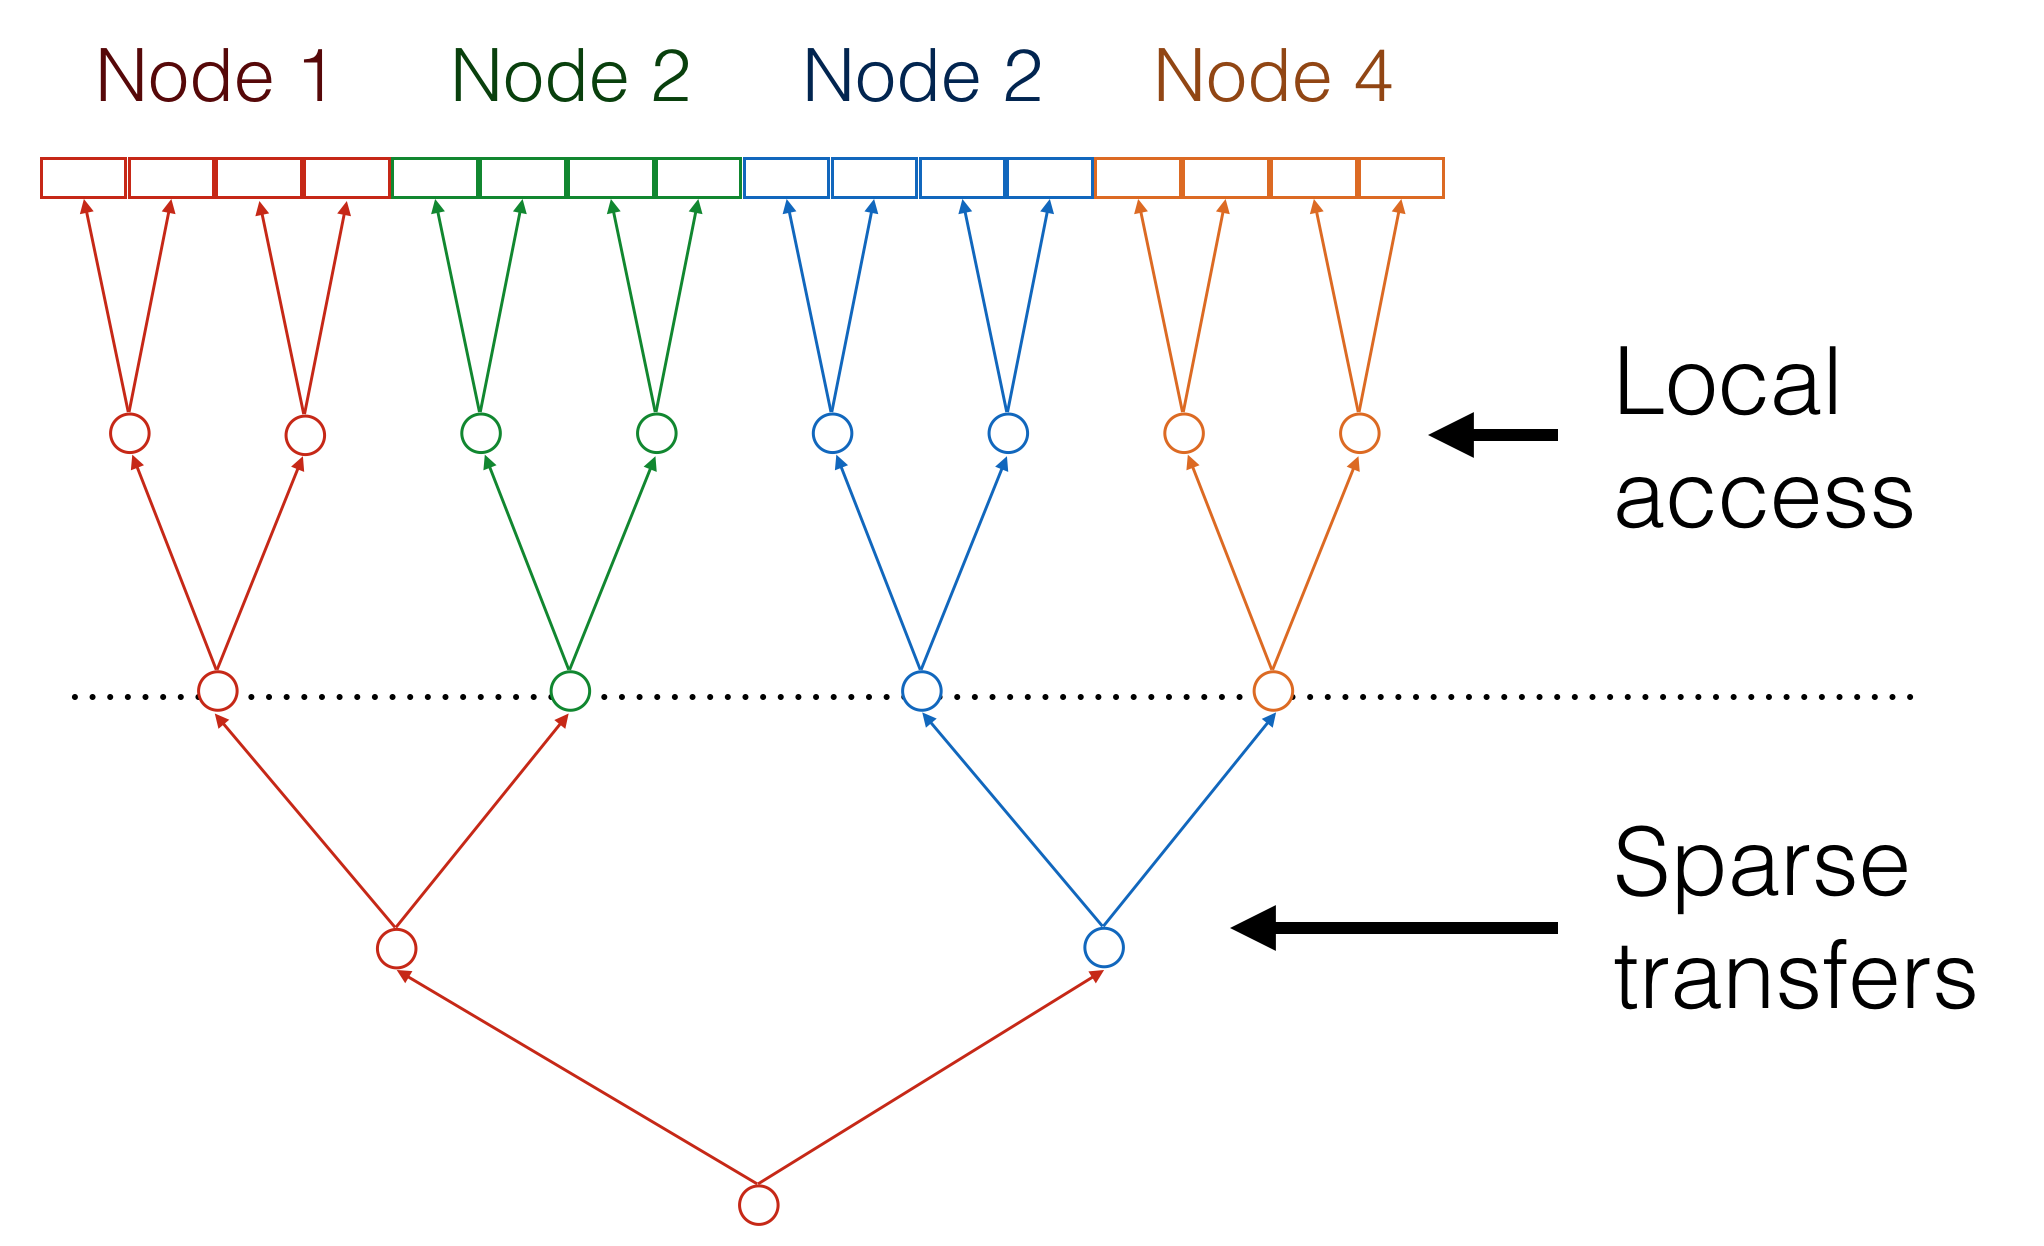
\includegraphics[width=0.6\textwidth]{figures/architecture}
\caption{%
An illustration of what makes partitioned global address space(PGAS) suitable for this algorithm.
The divide-and-conquer algorithm merges the tree by joining contiguous nodes from the ordered set.
As long as we constrain each thread to merge only subtrees in its local memory, all memory accesses will be local until the final $P - 1$ merge operations, where $P$ is the number of processors.
}
\label{fig:architecture}
\end{figure}

Once Shun \& Blelloch's code is written bottom-up, a simplified solution can be expressed elegantly, with only barrier-level synchronization:

\lstset{language=C}
\begin{minipage}{\linewidth}
\begin{lstlisting}
for (int step = 2; step < n * 2; step *= 2) {
  upc_forall (int start = 0; start < n; start += step; &Nodes[start]) {
    if (n - start >= step) tree_size = step;
    else tree_size = n - start;
    if (tree_size > step / 2) {
      middle = start + (step / 2) - 1;
      merge (Nodes, middle, middle + 1, index);
    }
    upc_barrier;
  }
}
\end{lstlisting}
\end{minipage}

\textbf{%
We needed to do the following to make this work feasibly:
set hard limits on the boundaries of each one.
Convert a cyclic buffer into a block-based shared memory buffer;
use upc\_barriers, to make sure that each level was only constructed after the last one was finished.
Work bottom-up instead of top-down.
Restrict to a static number of threads instead of dynamic
}

\begin{minipage}{\linewidth}
\begin{lstlisting}
for (int i = 0; i < n; i++) {
  thread = i / elements_per_thread;
  phase = i \% elements_per_thread;
  index[i] = thread + phase * THREADS;
}
\end{lstlisting}
\end{minipage}

We direct readers to the Shun \& Blelloch work for details on how merging is performed.

\section{Expected Performance}

\textbf{Explain this more and how we construct it}

We describe the expected performance here:
Assuming constant communication time $T_C$ and ``merge'' time $T_M$, the runtime for our multi-node algorithm can be estimated with this expression:

$\left( T_{ C }+T_{ M } \right) *(P-1)+\frac{T_M}{P}*(N-P)<T_{ M }*(N-1)$
$T_{ M } * (N-1)$

By simplifying a comparison with the Shun and Blelloch runtime, we find that our extension should achieve speedup as long as the following holds:
$T_C / T_M < N / P - 1$

\textbf{For example, this means that if it takes ten thousand times as long to communicate the entries necessary to perform a tree merge as to perform the merge itself, then there should be about ten thousand times as many nodes out of which to build the tree than there are processors.}

With around 150 ns measured for each merge and 250--3700 ns expected communication latency on NERSC's Edison machine,\footnote{\url{http://www.nersc.gov/users/computational-systems/edison/configuration/}} we do see performance improvements with more nodes.
Currently, improvement is sublinear with the number of nodes. 

\section{Results}

\begin{figure}
\centering
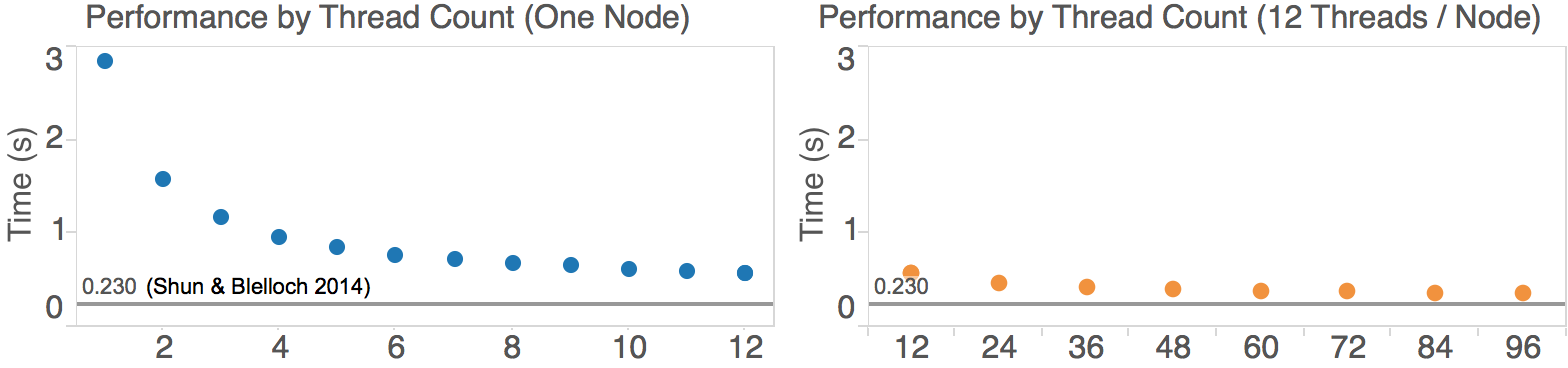
\includegraphics[width=0.9\textwidth]{figures/benchmarks}
\caption{%
Runtime of our Cartesian tree construction algorithm on a 10M text file, as we increase the number of threads and nodes.
The constant grey line is the Shun \& Blelloch (2014) baseline performance.
}
\label{fig:benchmarks}
\end{figure}

We see sub-linear evidence of strong scaling.
\textbf{%
Log-log plot of strong scaling.
Plot of weak scaling, with 500KB, 1MB, 2MB, 4MB, and 2 nodes.
}

\textbf{%
We also see evidence of weak scaling.
}

\textbf{%
Table with the following:
Timing of merge method and Cartesian tree methods with and without our improvements.
}

\begin{table*}[t]
\caption{Profiling diagnostics generated by \texttt{upc\_trace}}
\vspace{1.5ex}
\label{tab:profiling_diagnostics}
\centering
\begin{tabular}{ll}
\toprule
\textbf{Measure} & \textbf{Value} \\
\midrule
Trace time (per thread) & 70.22s \\ \midrule
Trace time (total, all threads) & 842.64s \\ \midrule
Time waiting for UPC barrier & 90.6s \\ \midrule
Number of memory 'get's & 1,363,142 \\ \midrule
Number of memory 'put's & 1,363,145 \\ \midrule
\end{tabular}
\end{table*}

My best guess at this point is that the lower performance is caused by the following:
\begin{itemize}
  \item Using too few threads.
        From the NERSC documentation on the Edison machine configuration, we found that each
        compute node has 12 cores with 1-2 threads each.
        \footnote{\url{http://www.nersc.gov/users/computational-systems/edison/configuration/}}
        Because of this, we assumed that 12 threads was the maximum number of threads to test before
        performance would degrade.
        However, we did not test this assumption.
        Particularly because there may be several memory accesses for each invocation of the merge
        method, it could be that threads wait during memory access.
        As the Shun \& Blelloch algorithm placed no explicit upper limit on the number of threads
        that could be running at any time, it's possible that more threads were running, resulting
        in a higher CPU utilization.
  \item Memory access.
        There are many more memory accesses than we might expect for this number of threads.
        The maximum it could be is the depth of both spines at each merge.
        There are only N merge operations that need to cross boundaries.
        \textbf{Insert the value for N here.}
        
  \item Time spent in \texttt{upc\_barrier}
  \item Time spent performing extra index lookup (we can compute the amount of time, given the number of merges)
  \item Time spent performing the shared buffer lookup
\end{itemize}

I have found it too challenging to find a resounding answer to my problem.
Line-by-line profiling seems unlikely to help.
Profiling adds a very large overhead for some relatively simple operations.
\texttt{gcov} is not supported to find out how often various code is invoked.
Adjustments to this problem could include:
\begin{itemize}
  \item Increasing the number of threads
  \item Using UPC locks instead of barriers on the elements around which merges are currently being 
        performed.
        All threads have to wait for the thread that takes the longest in order to proceed to the
        next level of depth of the merge.
        This may become particularly exaggerated as the height of each of the sub-trees becomes
        increasingly disparate as the merges continue.
        Instead of having a global barrier on each level, each merge can lock the elements that
        are at the root of each merge.
        Each subsequent level of merging will need to lock the same elements, so it has to wait
        for the sub-trees it is merging to have been completely merged.
        However, this would reduce the dependency of any given merge operation to waiting on just
        two previous merges instead of, in the worst case case, $N / 2 - 1$ merges.
  \item Extending the UPC source code to support block-based indexing instead of cyclic indexing.
        This would prevent the need to convert the index in each iteration from a cyclic index
        into a block-order index.
  \item Casting pointers to shared data types to pointers to private data for all merge operations
        until the merge needs to access nodes shared in other threads' memories.
        This reduces the need to convert shared memory addresses into a private address with every
        access, which likely causes many more computations for the first few levels of merges.
\end{itemize}

\textbf{%
What we did to profile the code, which includes:
method-level debugging,
performing tracing on the code---which is inherently pretty tough, unreliable.
}

Diagnostics of the poor performance include:
Memory access, UPC barriers.
Do the profiling once again, but with 2 nodes instead of 1.

We expect that the performance can be further improved by\ldots{}

\section{Conclusion}

Even with the maximum nodes and threads tested, we did not improve on Shun \& Blelloch's 
baseline performance, due to overhead we introduced with UPC\@.
While we did not achieve our goal of improving runtime to interactive speed, we did see speedup by introducing additional nodes.

\printbibliography{}

\end{document}
